\documentclass[sigconf]{acmart}

%% Using the option "anonymous" will produce "Anonymous Author(s)"
%% for double-anonymized review. Upon acceptance, remove this option
%% and set the authors' names and affiliations using the corresponding
%% commands.

%% CBSoft uses an ACM-like format without the ACM Reference block.
%% The following warning from acmart can be safely ignored:
%% "ACM reference format is mandatory for papers over one page."
\settopmatter{printacmref=false}
\renewcommand\footnotetextcopyrightpermission[1]{} % removes footnote with conference information in first column

%% CBSoft uses an ACM-like format without a copyright note.
\setcopyright{none}

%% These commands are for a PROCEEDINGS abstract or paper.
\acmConference[SBES 2026]{40th Brazilian Symposium on Software Engineering}{September 8--11, 2026}{São Paulo, SP, Brazil}

\usepackage{pgfplots}
\pgfplotsset{compat=1.18}
\usepackage{tikz}
\usetikzlibrary{shapes.geometric, arrows, positioning, calc}
\usepackage{graphicx}

% CBSoft uses an ACM-like format without CCS Concepts.
% The following warning from acmart can be safely ignored:
% "CCS concepts are mandatory for papers over two pages."

%% \BibTeX command to typeset BibTeX logo in the docs
\AtBeginDocument{
    \providecommand\BibTeX{{Bib\TeX}}
}

%% Only for papers written in PORTUGUESE: 
%% comment out the following three lines
%\renewcommand\abstractname{Resumo}
%\renewcommand\keywordsname{Palavras-chave}
%\renewcommand\refname{Referências}

%% end of the preamble, start of the body of the document source.

% \setlength{\parskip}{2pt plus 1pt minus 1pt}
% \setlength{\parskip}{2pt}


% ------------------------------------------------------------
% Authors: please make sure to read the checklist comments
% provided at the end of this document before submission.
% ------------------------------------------------------------
\begin{document}

%% The "title" command has an optional parameter,
%% allowing the author to define a "short title" to be used on the page 
%% headers.
\title{NoseSense: Benchmarking Tool}

%% The "author" command and its associated commands are used to define
%% the authors and their affiliations.
%% Of note is the shared affiliation of the first two authors, and the
%% "authornote" and "authornotemark" commands
%% used to denote shared contribution to the research.
\author{Magno Macedo}
\affiliation{
  \institution{Computer Institute, Federal University of Bahia}
  \city{Salvador}
  \country{Brazil}
}
\email{magnomiranda@ufba.br}

\author{Lucas Fraga}
\affiliation{
  \institution{Computer Institute, Federal University of Bahia}
  \city{Salvador}
  \country{Brazil}
}
\email{lucasfraga@ufba.br}

\author{Letícia Barreto}
\affiliation{
  \institution{Computer Institute, Federal University of Bahia}
  \city{Salvador}
  \country{Brazil}
}
\email{leticiabarreto@ufba.br}

\author{Tássio Virginio}
\affiliation{
  \institution{Computer Institute, Federal University of Bahia}
  \city{Salvador}
  \country{Brazil}
}
\email{tassio.virginio@ufba.br}

\author{Ivan Machado}
\affiliation{
  \institution{Computer Institute, Federal University of Bahia}
  \city{Salvador}
  \country{Brazil}
}
\email{ivan.machado@ufba.br}

%% By default, the full list of authors will be used on the page
%% headers. This list is often too long and will overlap
%% other information printed in the page headers. 
%% This command allows the author to define a more concise list
%% of authors' names for this purpose.
\renewcommand{\shortauthors}{Macedo et al.}
\renewcommand{\shorttitle}{NoseSense: Benchmarking Tool}

%% The abstract is a short summary of the work the paper presents.
\begin{abstract}

The rapid evolution of Large Language Models (LLMs), characterized by a shift from yearly to weekly advancements, has rendered traditional static evaluation studies quickly obsolete upon publication. In this fast-paced landscape, evaluation methodologies must be designed to enable immediate and continuous assessment of newly released models. Automated benchmarking has emerged as a practical solution, allowing LLMs to be evaluated and compared as soon as they become available.
% A rápida evolução dos Modelos de Linguagem de Grande Escala (LLMs), caracterizada por uma transição de avanços anuais para semanais, tornou os estudos tradicionais de avaliação estática rapidamente obsoletos logo após sua publicação. Neste cenário de ritmo acelerado, as metodologias de avaliação devem ser projetadas para viabilizar a análise imediata e contínua de modelos recém-lançados. O benchmarking automatizado emergiu como uma solução prática, permitindo que os LLMs sejam avaliados e comparados assim que se tornam disponíveis.
A wide range of benchmarks has been proposed to assess LLM capabilities across diverse application domains. However, there is a lack of targeted evaluation frameworks focusing on software engineering tasks related to test quality. In this context, we present an automated benchmarking tool designed to evaluate the accuracy of LLMs in identifying anti-patterns in test code, commonly referred to as Test Smells. Our approach enables scalable, reproducible, automated, and up-to-date assessment of LLM performance in this critical aspect of software quality.
% Uma ampla variedade de benchmarks tem sido proposta para avaliar as capacidades dos LLMs em diversos domínios de aplicação. No entanto, há uma escassez de frameworks de avaliação direcionados com foco em tarefas de engenharia de software relacionadas à qualidade de testes. Neste contexto, apresentamos uma ferramenta automatizada de benchmarking projetada para avaliar a acurácia de LLMs na identificação de antipadrões em código de teste, comumente denominados Test Smells. Nossa abordagem viabiliza uma avaliação escalável, reprodutível, automatizada e atualizada do desempenho dos LLMs neste aspecto crítico da qualidade de software.
The tool demonstration video can be found on zenodo \\\url{https://zenodo.org/records/20277258} and youtube \url{https://youtu.be/D0o77YuM_Xs}.
\end{abstract}
%% Keywords. The author(s) should pick words that accurately describe
%% the presented work. Separate the keywords with commas.
\keywords{LLM, Benchmarks, Tools, Test Smells}

%% This command processes the author, affiliation, and title
%% information and builds the first part of the formatted document.
%% "frenchspacing" avoids an additional space after a period at the end of a sentence.
\frenchspacing
\maketitle

\section{Introduction}
The vast presence of digital systems in modern society has established robustness and reliability as fundamental pillars of Software Engineering. In this context, maintaining high-quality test suites is imperative to mitigate failures and reduce long term operational costs. However, the effectiveness of these tests is frequently compromised by design anti-patterns called test smells that do not impair code functionality, but degrade its readability, maintainability, and evolution \cite{Virginio2019}.

% A onipresença de sistemas digitais na sociedade moderna estabeleceu a robustez e a  {confiabilidade} como pilares fundamentais da Engenharia de Software. Nesse cenário, a manutenção de suítes de teste de alta qualidade é imperativa para mitigar falhas e reduzir custos operacionais em longo prazo. Entretanto, a eficácia desses testes é frequentemente comprometida pelos denominados  {test smells}, antipadrões de design que, embora não impeçam o funcionamento do código, degradam sua legibilidade, manutenibilidade e  evolução\cite{Virginio2019}. 

The search for automated solutions to identify and refactor these anti-patterns has found a promising yet complex path in Large Language Models (LLMs) \cite{alves2025quality,lucas2024evaluating,wu2024ismell}. This complexity stems primarily from a critical methodological challenge: the temporal volatility of experimental results. The innovation cycle of LLMs has been so accelerated that comparative studies of benchmarks tend to become saturated and obsolete even before their publication \cite{allen2026well,ott2022mapping}. In the interval required to conclude a rigorous investigation, the release of new model iterations often invalidates static benchmarks, turning the state of the art into a moving target, which undermines the ability to use the study's findings as a foundation for further research or industrial application.

% A busca por soluções automatizadas para identificar e refatorar esses antipadrões tem encontrado nas LLMs ( {Large Language Models}) um caminho promissor, porém complexo \cite{}. Essa complexidade reside, primordialmente, em um desafio metodológico crítico: a volatilidade temporal dos resultados experimentais. O ciclo de inovação das LLMs é tão acelerado que estudos comparativos voltados à detecção de  {test smells} tendem a se tornar obsoletos antes mesmo de sua publicação \cite{}. No intervalo necessário para concluir uma investigação rigorosa, o lançamento de novas iterações de modelos costuma invalidar  {benchmarks} estáticos, transformando o estado da arte em um alvo móvel, o que compromete utilizar os resultados e os achados do estudo como base de outros estudos e para a utilização na industria.

To mitigate this issue, we present NoseSense, a dynamic benchmarking tool designed to simultaneously evaluate the performance of multiple LLMs in detecting test smells. To enable scalable and reproducible evaluation, the tool operationalizes this detection task through a structured multiple-choice benchmark: each sample presents a code snippet containing a test smell, and the model must identify which smell is present by selecting among a set of predefined options. This controlled format ensures that model responses can be automatically verified against a ground-truth oracle, allowing rigorous measurement of each LLM's ability to recognize test smell patterns. 

% NoseSense specifically targets this classification capability, providing a controlled and reproducible setting in which the model's semantic understanding of test smell definitions can be rigorously measured. 
Our project provides a robust solution that addresses the limitations of traditional studies on this topic, which often become obsolete during the lengthy writing and publication process. Instead of time-consuming longitudinal analyses, the project prioritizes rapid, practical validation, enabling real-time comparisons of the most current models. The necessity for tools like NoseSense is reinforced by the high prevalence of anti-patterns in real-world systems \cite{alves2025quality}, empirical studies indicate that between 18\% to 26\% of test suites are free of test smells \cite{Bavota2012,sast2026}. Thus, NoseSense serves as a diagnostic instrument for the semantic classification capability of LLMs with respect to test code quality, providing continuously updated metrics that keep pace with the industry's rapid technological evolution.
% Para mitigar esse problema, apresentamos o   {NoseSense}, uma ferramenta de  {benchmarking} dinâmico projetada para avaliar a performance de múltiplas LLMs simultaneamente na detecção  de test smells, ou seja, na qualidade do código de teste. Nosso projeto trouxe uma solução robusta que substitui estudos sobre o tema (qualidade de código de testes) por llms, os quais precisam passar por  todo um processo de escrita e publicação já são publicados defasados. Além disso em vez de análises longitudinais demoradas, o projeto prioriza uma validação prática e rápida, permitindo a comparação de modelos mais atuais em tempo real. A necessidade de ferramentas como o NoseSense é evidenciada pela alta prevalência de antipadrões em sistemas reais, estudos empíricos indicam que apenas 18\% das suítes de teste estão livres de test smells\cite{Bavota2012}. Assim, o   {NoseSense} atua como uma ferramenta de diagnóstico para a eficácia analítica dessas inteligências artificiais em verificar a qualidade dos códigos de testes, fornecendo métricas atualizadas conforme a evolução desenfreada da tecnológica do setor. 
% \textbf{Contributions.} The primary contributions of this paper are:
% \begin{itemize}
%     \item {NoseSense}, a dynamic benchmarking tool designed to simultaneously evaluate the performance of multiple Large Language Models (LLMs) in detecting test smells.
%     \item {A pragmatic evaluation methodology} that overcomes the rapid obsolescence of traditional static studies, providing a continuous metrology instrument for AI code analysis capabilities.
%     \item{A comprehensive visualization and data consolidation environment} that automatically processes LLM outputs, simplifying the interpretation of complex benchmarking results for researchers.
% \end{itemize}
% The remainder of this paper is organized as follows. Section~\ref{sec:test_smells} introduces the test smell categories used in the evaluation. Section~\ref{sec:related_work} positions NoseSense in relation to existing tools and studies. Section~\ref{sec:nosesense} details the tool's features, architecture, and operational workflow. Section~\ref{sec:experimentacao} presents a proof-of-concept experiment demonstrating the tool's capabilities. Finally, Section~\ref{sec:conclusao} discusses limitations, future directions, and concluding remarks.
% O restante deste artigo está organizado da seguinte forma. A Seção~\ref{sec:test_smells} apresenta as categorias de test smells utilizadas na avaliação. A Seção~\ref{sec:related_work} posiciona o NoseSense em relação a ferramentas e estudos existentes. A Seção~\ref{sec:nosesense} detalha as funcionalidades, arquitetura e fluxo operacional da ferramenta. A Seção~\ref{sec:experimentacao} apresenta um experimento de prova de conceito. Por fim, a Seção~\ref{sec:conclusao} discute limitações, direções futuras e considerações finais.
\section{Test Smells}
\label{sec:test_smells}

% The theoretical foundation regarding the degradation of quality in test codes traces back to the original work by Deursen et al.~\cite{Deursen01}. The authors established the concept of test smells as symptoms of suboptimal code that, although not preventing the functional execution of tests, severely compromise the maintainability, reliability, and diagnostic capability of validation suites. These anti-patterns increase the difficulty level of software maintenance and can mask latent defects in the production code \cite{Virginio2019, bavota2015test}.
% A fundamentação teórica acerca da degradação da qualidade em códigos de teste remete ao trabalho original de Deursen et al.~\cite{Deursen01}. Os autores estabeleceram o conceito de  {test smells} como sintomas de códigos subótimos que, embora não impeçam a execução funcional dos testes, comprometem severamente a manutenibilidade, a confiabilidade e a capacidade diagnóstica das suítes de validação. Estes antipadrões elevam o nível de dificuldade de manutenção do software e podem mascarar defeitos latentes no código de produção \cite{Virginio2019}.
Van Deursen et al. \cite{Deursen01} argue that test smells possess their own taxonomy and corresponding remedies, identifying eleven distinct types in their seminal work. Later studies expanded this taxonomy by proposing additional smell types and examining their distribution and co-occurrence patterns \cite{peruma2019distribution,virginio2020jnose,santana2025empirical,Virginio2019,bavota2015test,Deursen01}. To evaluate the effectiveness of NoseSense, we selected a set of 10 test smells, detailed below:

% Van Deursen et al. \cite{Deursen01} argumentam que os odores de teste possuem sua própria taxonomia e soluções correspondentes, identificando onze tipos distintos em seu trabalho seminal. Estudos posteriores expandiram essa taxonomia, propondo tipos adicionais de odores e examinando seus padrões de distribuição e coocorrência \cite{peruma2019distribution,virginio2020jnose,santana2025empirical}. Para avaliar a eficácia do NoseSense, selecionamos um conjunto de 10 odores de teste, detalhados abaixo:

% Para a avaliação da eficácia do   {NoseSense}, selecionamos um conjunto de 10  {test smells}, detalhados a seguir:

    \textbf{Assertion Roulette (AR):}
    Occurs when a test method encapsulates multiple assertions without explanatory messages.
    % Ocorre quando um método de teste encapsula múltiplas asserções sem mensagens explicativas. Esta prática obscurece a rastreabilidade da falha, em caso de interrupção, torna-se custoso identificar qual condição específica foi violada, prejudicando o tempo de depuração e a interpretabilidade do erro \cite{}.

    \textbf{Conditional Test Logic (CTL):}
    Characterized by the presence of control structures in the test body.
    % Caracteriza-se pela presença de estruturas de controle (como \texttt{if}, \texttt{for} ou \texttt{while}) no corpo do teste. Tais construções elevam a complexidade ciclomática, podendo introduzir comportamentos não determinísticos e dificultar a verificação de todos os caminhos de execução possíveis \cite{}.

    \textbf{Duplicate Assert (DA):} 
    Manifests through the repetition of assertions that validate identical states or conditions within the same test scope.
    % Manifesta-se através da repetição de asserções que validam estados ou condições idênticas dentro do mesmo escopo de teste. Esta redundância infla o volume de código e aumenta o esforço de manutenção sem proporcionar incrementos reais na cobertura \cite{}.

    \textbf{Eager Test (ET):}
    Occurs when a single test method attempts to verify multiple functionalities or production class methods simultaneously.
    % Ocorre quando um único método de teste tenta verificar múltiplas funcionalidades ou métodos da classe de produção simultaneamente. É uma violação direta do  {Princípio de Responsabilidade Única} (SRP), resultando em testes densos e de difícil compreensão \cite{}.

    \textbf{Exception Catching Throwing (ECT):}
    Refers to the improper use of \texttt{try-catch} blocks to catch exceptions that should be propagated to the test framework.
    % Refere-se ao uso indevido de blocos \texttt{try-catch} para capturar exceções que deveriam ser propagadas ao  {framework} de testes. Esta prática pode levar a falsos positivos ou ocultar a real natureza de falhas sistêmicas \cite{}.

    \textbf{Ignored Test (IT):}
    Identifies tests that were explicitly disabled (e.g., \texttt{@Ignore} annotation).
    % Identifica testes que foram explicitamente desativados (ex: anotação \texttt{@Ignore}). Representam uma forma de dívida técnica, indicando validações obsoletas que deixam o sistema vulnerável a regressões não detectadas \cite{}.

    \textbf{Magic Number (MN):}
    Consists of using literal numbers without explicit semantic context in assertions.
    % Consiste na utilização de números literais sem contexto semântico explícito em asserções. A ausência de constantes nomeadas obscurece a intenção da validação e exige que o desenvolvedor deduza o significado do valor arbitrário \cite{}.

    \textbf{Sensitive Equality (SE):}
    Occurs when the equality criterion relies on the textual representation (\texttt{toString}) of complex objects.
    % Ocorre quando o critério de igualdade baseia-se na representação textual (\texttt{toString}) de objetos complexos. Torna o teste excessivamente frágil, pois alterações triviais na formatação da saída podem causar falhas, independentemente da integridade da lógica.

    \textbf{Unknown Test (UT):}
    Represents methods that execute production code but lack assertions.
    % Representam métodos que executam o código de produção, mas carecem de asserções ( {assertion-less tests}). Embora contribuam para métricas nominais de cobertura, são ineficazes por não validarem estados reais \cite{}.

    \textbf{Verbose Test (VT):}
    Characterized by excessively long test methods.
    \vspace{-10px}
    % Caracteriza-se por métodos de teste excessivamente extensos. A verbosidade é um indicador de que o caso de teste está tentando validar comportamentos em exagero ou que os procedimentos de configuração ( {setup}) estão mal projetados \cite{}.


% \section{Related Work}
% \label{sec:related_work}

% Several studies have explored both static analysis tools and LLM-based approaches for test smell detection \cite{virginio2020jnose, lucas2024evaluating, wu2024ismell, santana2024empirical}. While these works provide valuable insights into model capabilities and detection heuristics, they do not offer dedicated software tools or reusable infrastructure for systematically evaluating LLMs. 
% The rapid evolution of artificial intelligence demands continuous and dynamic evaluation mechanisms, which cannot be efficiently supported by manual executions or ad-hoc experimental setups.
% Diversos estudos exploraram tanto ferramentas de análise estática quanto abordagens baseadas em LLMs para detecção de test smells \cite{virginio2020jnose, lucas2024evaluating, wu2024ismell}. Embora esses trabalhos forneçam insights valiosos sobre as capacidades dos modelos e heurísticas de detecção, eles não oferecem ferramentas de software dedicadas ou infraestrutura reutilizável para a avaliação sistemática de LLMs. A rápida evolução da inteligência artificial exige mecanismos de avaliação contínuos e dinâmicos, que não podem ser eficientemente suportados por execuções manuais ou configurações experimentais ad-hoc.

% In this context, NoseSense introduces a novel approach by providing an automated and reusable pipeline that allows any newly released model to be evaluated immediately. While tools like JNose and RAIDE \cite{virginio2020jnose, santana2024empirical} focus on collecting, detecting and refactoring test smells directly from source code, NoseSense serves a different purpose: it is designed as a metrology instrument to evaluate and determine which LLMs perform best at this detection task. By offering a reproducible benchmarking infrastructure, it enables continuous monitoring of AI capabilities over time. Furthermore, while rule-based tools like JNose provide high precision within their hardcoded heuristics, making them ideal for constructing deterministic oracles, they lack semantic understanding. Static analyzers are notoriously rigid and prone to false positives when test codes deviate from predefined structural patterns. In contrast, LLM-based approaches offer flexible, context-aware analysis capable of interpreting developer intent, handling nuanced anti-patterns, and immediately generating refactored code. Therefore, NoseSense does not position LLMs as mere replacements for static tools, but aims to evaluate their maturity in achieving semantic comprehension of software quality.
% Neste contexto, o NoseSense introduz uma nova abordagem ao fornecer um \textit{pipeline automatizado e reutilizável} que permite que qualquer modelo recém-lançado seja avaliado imediatamente. Enquanto ferramentas como o JNose focam em coletar e detectar test smells diretamente do código-fonte, o NoseSense serve a um propósito diferente: foi projetado como um \textit{instrumento de metrologia} para avaliar e determinar quais LLMs se saem melhor nessa tarefa de detecção. Ao oferecer uma infraestrutura de benchmarking reprodutível, ele permite o monitoramento contínuo das capacidades da IA ao longo do tempo. Além disso, embora ferramentas baseadas em regras como o JNose forneçam alta precisão dentro de suas heurísticas fixas --- tornando-as ideais para construir oráculos determinísticos ---, elas carecem de compreensão semântica. Analisadores estáticos são notoriamente rígidos e propensos a falsos positivos quando o código de teste se desvia dos padrões estruturais predefinidos. Em contraste, abordagens baseadas em LLM oferecem análises flexíveis e sensíveis ao contexto, capazes de interpretar a intenção do desenvolvedor, lidar com antipadrões sutis e gerar imediatamente o código refatorado. Portanto, o NoseSense não posiciona os LLMs como meros substitutos das ferramentas estáticas, mas visa avaliar sua maturidade em alcançar a compreensão semântica da qualidade do software.

\section{NoseSense}
% \section{O   {NoseSense}}
\label{sec:nosesense}

% \begin{figure}[H]
%     \centering
%     \includegraphics[width=1\linewidth]{nosesense2.png}
%     \caption{NoseSense main screen}
%     \label{fig:main_screen}
% \end{figure}
%as seen in Figure \ref{fig:main_screen},
NoseSense provides a controlled and systematic environment for evaluating the capability of LLMs in detecting test smells. To ensure the statistical rigor of the analyses, the tool integrates an oracle composed of 1,000 code instances, comprising 100 samples for each of the 10 test smells selected and described in Section~\ref{sec:test_smells}. This oracle is used to assess the precision and diagnostic accuracy of the evaluated artificial intelligence models. The following subsections detail the tool's features, systemic architecture, and operational workflow. The oracle dataset focuses on Java test code and it happens for two main reasons: first, this language remains the most widely studied in the test smell literature~\cite{Deursen01, Virginio2019, virginio2020jnose, peruma2019distribution}; second, JNose, the static analysis tool utilized to extract and validate the ground-truth samples for our oracle, was exclusively designed to operate on Java projects. This methodological choice ensures compatibility with established definitions and provides robust empirical foundations.
% Esta seção apresenta o NoseSense, uma ferramenta computacional concebida para prover um ambiente controlado e sistemático à avaliação da capacidade de LLMs na detecção de test smells. Para assegurar o rigor estatístico das análises, a ferramenta integra um oráculo composto por 1.000 instâncias de código, contemplando 100 amostras para cada um dos 10 test smells selecionados e descritos na Seção~\ref{sec:test_smells}. Este oráculo é utilizado para aferir a precisão e a acurácia diagnóstica dos modelos de inteligência artificial avaliados. Nas subseções seguintes, detalham-se as funcionalidades, a arquitetura sistêmica e o fluxo operacional da ferramenta.
%O dataset oráculo foca em código de teste Java e isso acontece por duas razões principais: primeiro, esta linguagem permanece a mais amplamente estudada na literatura de test smells~\cite{Deursen01, Virginio2019, virginio2020jnose, peruma2019distribution}; segundo, o JNose---ferramenta de análise estática utilizada para extrair e validar as amostras de ground-truth para o nosso oráculo---foi projetado exclusivamente para operar em projetos Java. Essa escolha metodológica garante compatibilidade com definições estabelecidas e fornece fundamentos empíricos robustos.


\subsection{Features}
% \subsection{Funcionalidades}
\label{subsec:funcionalidades}

NoseSense was designed with a set of features that cover the entire model evaluation lifecycle, from configuration to results analysis:
% O {NoseSense} foi projetado com um conjunto de funcionalidades que abrangem todo o ciclo de vida da avaliação de modelos, desde a configuração até a análise dos resultados:

    \textbf{Provider and Model Registration:} Enables the inclusion of multiple AI platforms with their credentials, allowing quick adoption of newly released models.
    % \item \textbf{Cadastro de provedores e modelos:} Viabiliza o registro de múltiplas plataformas de IA e credenciais, garantindo a rápida adição de novos modelos.
    
    \textbf{Automated Benchmark Execution:} Evaluates multiple LLMs simultaneously against an oracle of 1,000 test smell samples, with real-time monitoring and interruption capabilities.
    % \item \textbf{Execução automatizada do benchmark:} Avalia simultaneamente múltiplas LLMs contra o oráculo de 1.000 amostras, com monitoramento em tempo real e possibilidade de interrupção.
    
    \textbf{Analytical Dashboard:} Consolidates results into graphical visualizations (bar, pie, and radar charts) to easily compare overall accuracy and specific capabilities.
    % \item \textbf{Dashboard analítico:} Consolida dados em visualizações gráficas (barras, pizza e radar) para fácil comparação de acurácia e capacidades específicas.
    
    \textbf{Results Persistence and Export:} Automatically stores evaluation history in a relational database and allows full CSV exports to ensure experiment reproducibility.
    % \item \textbf{Persistência e exportação de resultados:} Armazena automaticamente os ensaios em banco de dados e permite exportação para CSV, assegurando reprodutibilidade.


\subsection{System Architecture}
% \subsection{Arquitetura do Sistema}
\label{subsec:arquitetura}

NoseSense adopts a client-server architecture based on the decoupling of a backend and a reactive user interface. This layered organization ensures that the model orchestration logic operates independently from the presentation layer, promoting high maintainability, simplicity and ecosystem scalability \cite{richards2020fundamentals}. 
% O   {NoseSense} adota uma arquitetura cliente-servidor fundamentada no desacoplamento entre um  {backend} e uma interface de usuário reativa. Essa organização em camadas assegura que a lógica de orquestração dos modelos opere de forma independente da camada de apresentação, promovendo alta manutenibilidade e escalabilidade do ecossistema \cite{}. 


\begin{figure}[htb]
    \centering
    \resizebox{\columnwidth}{!}{%
    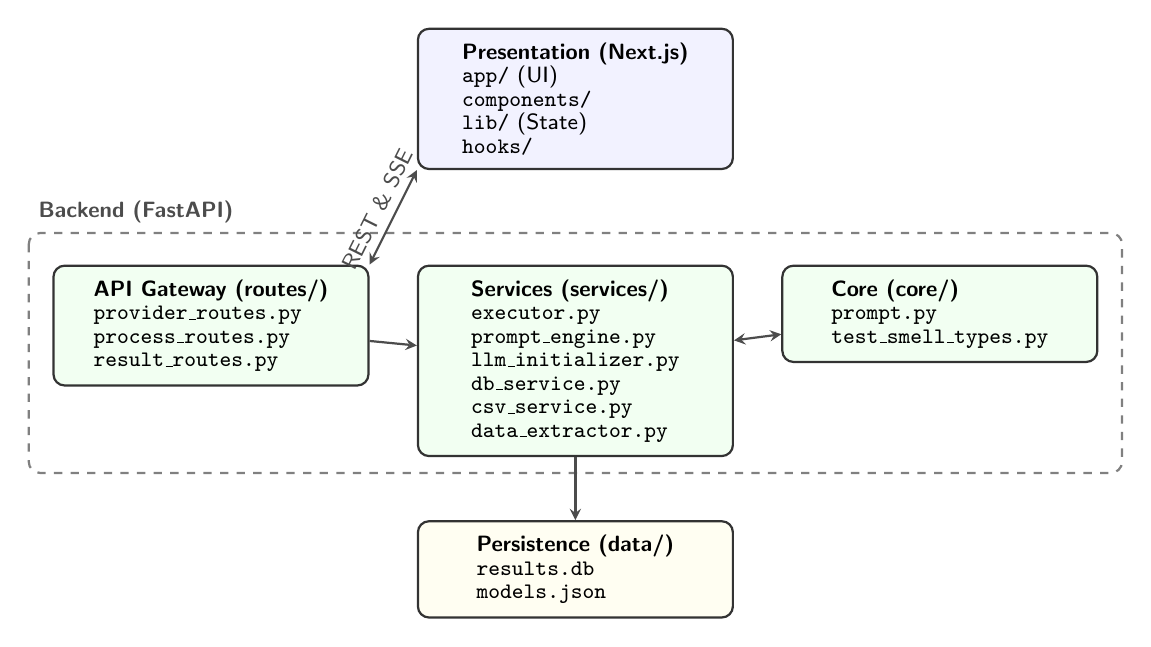
\begin{tikzpicture}[
        >=stealth,
        node distance=0.6cm,
        box/.style={
            rectangle, draw=black!80, fill=gray!5, thick, rounded corners, 
            inner sep=5pt, align=left, font=\sffamily\footnotesize, 
            minimum width=4.0cm
        },
        arrow/.style={->, thick, color=black!70},
        bidir/.style={<->, thick, color=black!70}
    ]

    % --- Nodes ---
    \node[box, fill=blue!5] (presentation) {
        \textbf{Presentation (Next.js)} \\[-1pt]
        \texttt{app/} (UI)\\[-1pt]
        \texttt{components/}\\[-1pt]
        \texttt{lib/} (State)\\[-1pt]
        \texttt{hooks/}
    };

    \node[box, fill=green!5, below=1.2cm of presentation] (services) {
        \textbf{Services (services/)} \\[-1pt]
        \texttt{executor.py}\\[-1pt]
        \texttt{prompt\_engine.py}\\[-1pt]
        \texttt{llm\_initializer.py}\\[-1pt]
        \texttt{db\_service.py}\\[-1pt]
        \texttt{csv\_service.py}\\[-1pt]
        \texttt{data\_extractor.py}
    };

    \node[box, fill=green!5, left=0.6cm of services.north west, anchor=north east] (gateway) {
        \textbf{API Gateway (routes/)} \\[-1pt]
        \texttt{provider\_routes.py}\\[-1pt]
        \texttt{process\_routes.py}\\[-1pt]
        \texttt{result\_routes.py}
    };
    
    \node[box, fill=green!5, right=0.6cm of services.north east, anchor=north west] (core) {
        \textbf{Core (core/)} \\[-1pt]
        \texttt{prompt.py}\\[-1pt]
        \texttt{test\_smell\_types.py}
    };

    \node[box, fill=yellow!5, below=0.8cm of services] (db) {
        \textbf{Persistence (data/)} \\[-1pt]
        \texttt{results.db}\\[-1pt]
        \texttt{models.json}
    };

    % --- Backend Background ---
    \draw[dashed, draw=black!50, thick, rounded corners] 
        ($(gateway.north west) + (-0.3, 0.4)$) rectangle ($(core.east |- services.south) + (0.3,-0.2)$);
    \node[font=\sffamily\bfseries\footnotesize, color=black!70, anchor=south west] at ($(gateway.north west) + (-0.3, 0.4)$) {Backend (FastAPI)};

    % --- Connections ---
    \draw[bidir] (presentation.south west) -- node[above, sloped, font=\footnotesize\sffamily] {REST \& SSE} (gateway.north east);
    \draw[arrow] (gateway) -- (services);
    \draw[bidir] (services) -- (core);
    \draw[arrow] (services) -- (db);
    
    \end{tikzpicture}%
    }
    \caption{NoseSense System Architecture Diagram.}
    % \caption{Diagrama de Arquitetura do {NoseSense}.}
    \label{fig:arquitetura_uml}
    \vspace{-10px}
\end{figure}


As detailed in Figure~\ref{fig:arquitetura_uml}, the system's core, located in the \texttt{/backend} directory, utilizes the \texttt{FastAPI} framework\footnote{\url{https://fastapi.tiangolo.com/}} , selected for its asynchronous nature. The structure is subdivided into logical layers ranging from data reception to persistence. Interaction begins at the Routes Layer (API Gateway), situated in \texttt{routes/}, which acts as the entry point and isolates responsibilities into specific domains: provider management (\texttt{provider\_routes.py}), analysis execution (\texttt{process\_routes.py}), and history retrieval (\texttt{result\_routes.py}).




% Conforme detalhado na Figura~\ref{fig:arquitetura_uml}, o núcleo do sistema, localizado no diretório \texttt{/backend}, utiliza o  {framework} \texttt{FastAPI} (v0.136.1), selecionado por sua natureza assíncrona. A estrutura é subdividida em camadas lógicas que abrangem desde a recepção de dados até a sua persistência. A interação inicia-se pela Camada de Rotas ( {API Gateway}), situada em \texttt{routes/}, que atua como ponto de entrada e isola as responsabilidades em domínios específicos: gerenciamento de provedores (\texttt{provider\_routes.py}), execução de análises (\texttt{process\_routes.py}) e recuperação de históricos (\texttt{result\_routes.py}).

Below this interface, the system's business rules reside in the Services Layer (\texttt{services/}). At this level, the \texttt{executor.py} component manages call concurrency to avoid rate limit penalties, while \texttt{prompt\_engine.py} applies randomization rules to the multiple-choice options to ensure the randomness of the tests. Instance initialization, performed via LangChain, is isolated in the \texttt{llm\_\allowbreak initializer.py} module, ensuring the modularity of the inference engine. Complementarily, the Core Layer encapsulates the essential definitions of test smells in the \texttt{core/} directory, centralizing the application's domain.
% Abaixo dessa interface, as regras de negócio do sistema residem na Camada de Serviços (\texttt{services/}). Neste nível, o componente \texttt{executor.py} gerencia a concorrência das chamadas para evitar penalidades de  {rate limit}, enquanto o \texttt{prompt\_engine.py} aplica regras de randomização nas opções de múltipla escolha para assegurar a randomicidade dos testes. A inicialização de instâncias, realizada via  {LangChain}, é isolada no módulo \texttt{llm\_initializer.py}, garantindo a modularidade do motor de inferência. Complementarmente, a Camada  {Core} encapsula as definições essenciais dos  {test smells} no diretório \texttt{core/}, centralizando o domínio da aplicação.

Finally, information management occurs in the Persistence Layer (\texttt{data/}), which adopts a hybrid approach: configuration metadata and credentials are kept in \texttt{JSON} files for flexibility, while evaluation results are persisted in a relational database. This strategy ensures referential data integrity, facilitates metric extraction, and enables automated export through the \texttt{csv\_service.py} service.
% Por fim, a gestão da informação ocorre na Camada de Persistência (\texttt{data/}), que adota uma abordagem híbrida: metadados de configuração e credenciais são mantidos em arquivos \texttt{JSON} pela sua flexibilidade, enquanto os resultados de avaliações são persistidos em um banco de dados relacional. Essa estratégia assegura a integridade referencial dos dados, facilita a extração de métricas e viabiliza a exportação automatizada por meio do serviço \texttt{csv\_service.py}.


Complementing the backend, the system's presentation layer (\texttt{/frontend}) is built with \texttt{Next.js}\footnote{\url{https://nextjs.org/}} and \texttt{React}\footnote{\url{https://react.dev/}} technologies, aiming to provide a fluid and data-driven User Experience. The structuring of pages and visual components (\texttt{app/}) employs the App Router paradigm to manage navigation and global layout, significantly optimizing rendering.
% A interface do sistema (\texttt{/frontend}), conforme ilustrado na Figura~\ref{fig:arquitetura_uml}, é construída com as tecnologias \texttt{Next.js} (v16.1.6) e \texttt{React}, visando proporcionar uma experiência de usuário ( {UX}) fluida e orientada a dados. A estruturação das páginas e componentes visuais (\texttt{app/}) emprega o paradigma  {App Router} para gerenciar a navegação e o  {layout} global, otimizando de forma significativa a renderização.

% In addition to the visual structure, application state management and reactivity are centrally controlled by local hooks and the global store (\texttt{lib/store.ts}). This organization coordinates asynchronous data consumption, ensuring that the analytical dashboard and visual indicators reflect server updates in real time without penalizing browser performance.
% Em complemento à estrutura visual, a gestão de estado e a reatividade da aplicação são controladas de forma centralizada pelos  {hooks} locais e pela  {store} global (\texttt{lib/store.ts}). Essa organização coordena o consumo assíncrono de dados, garantindo que o  {dashboard} analítico e os indicadores visuais reflitam as atualizações do servidor em tempo real, sem penalizar o desempenho do navegador.


To ensure the cohesion of the ecosystem illustrated in Figure~\ref{fig:arquitetura_uml}, the communication between frontend and backend utilizes the \texttt{REST} approach for static configurations and registrations. However, for the critical and prolonged process of test smell analysis, the system employs the Server-Sent Events (SSE) protocol. 
% This architecture establishes a low-latency, unidirectional channel, allowing the backend to instantly transmit partial results and progress tracking to the interface. This architectural decision eliminates the overhead of inefficient iterative polling and ensures a dynamic and responsive visualization of the benchmark.
% Para garantir a coesão do ecossistema ilustrado na Figura~\ref{fig:arquitetura_uml}, a comunicação entre  {frontend} e  {backend} utiliza a abordagem \texttt{REST} para configurações e cadastros estáticos. No entanto, para o processo crítico e prolongado de análise de  {test smells}, o sistema emprega o protocolo  {Server-Sent Events} (SSE). Essa arquitetura estabelece um canal unidirecional de baixa latência, permitindo que o  {backend} transmita resultados parciais e acompanhamento do progresso instantaneamente para a interface. Essa decisão arquitetural elimina a sobrecarga de verificações iterativas ( {polling}) ineficientes e assegura uma visualização dinâmica e responsiva do  {benchmark}.

% \subsection{Operational Workflow}
% The operation of NoseSense is structured in a linear and deterministic pipeline, designed to ensure that model evaluation occurs in an isolated and monitorable manner. The operational workflow, detailed in Figure~\ref{fig:nosesense_workflow}, is divided into the following stages:
% O funcionamento do   {NoseSense} é estruturado em um  {pipeline} linear e determinístico, projetado para garantir que a avaliação dos modelos ocorra de forma isolada e monitorável. O fluxo operacional, detalhado na Figura~\ref{fig:nosesense_workflow}, é dividida nas seguintes etapas:

\begin{figure*}[bth]
    \centering
    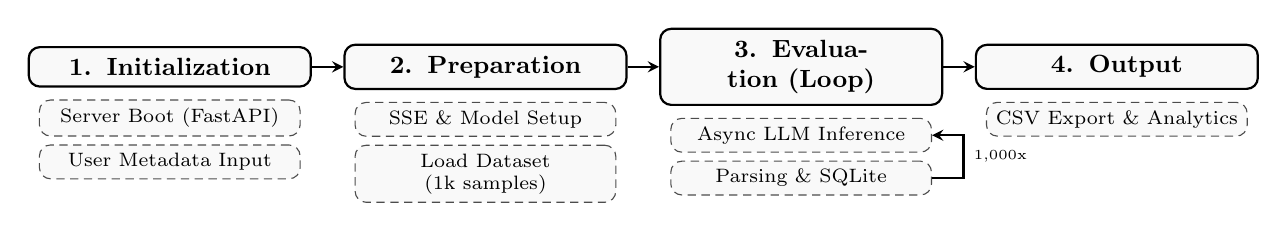
\begin{tikzpicture}[
        node distance=0.5cm and 0.4cm,
        stage/.style={rectangle, draw=black!110, fill=gray!5, thick, rounded corners, inner sep=4pt, text centered, font=\small\bfseries, text width=3.3cm},
        substep/.style={rectangle,
        draw=black!70,
        fill=gray!5,
        thin,
        densely dashed,
        rounded corners,
        inner sep=3pt,
        text width=3.1cm,
        align=center,
        font=\scriptsize},
        arrow/.style={thick, ->, >=stealth}
    ]

    % --- STAGE 1 ---
    \node (s1) [stage] {1. Initialization};
    \node (s1a) [substep, below=0.15cm of s1] {Server Boot (FastAPI)};
    \node (s1b) [substep, below=0.1cm of s1a] {User Metadata Input};

    % --- STAGE 2 ---
    \node (s2) [stage, right=of s1] {2. Preparation};
    \node (s2a) [substep, below=0.15cm of s2] {SSE \& Model Setup};
    \node (s2b) [substep, below=0.1cm of s2a] {Load Dataset (1k samples)};

    % --- STAGE 3 ---
    \node (s3) [stage, right=of s2] {3. Evaluation (Loop)};
    \node (s3a) [substep, below=0.15cm of s3] {Async LLM Inference};
    \node (s3b) [substep, below=0.1cm of s3a] {Parsing \& SQLite};

    % --- STAGE 4 ---
    \node (s4) [stage, right=of s3] {4. Output};
    \node (s4a) [substep, below=0.15cm of s4] {CSV Export \& Analytics};

    % --- ARROWS ---
    \draw [arrow] (s1) -- (s2);
    \draw [arrow] (s2) -- (s3);
    \draw [arrow] (s3) -- (s4);

    % --- LOOP ARROW ---
    \draw [arrow] (s3b.east) -- ++(0,-0.0) -- ++(0.4,0) |- node[pos=0.25, right, font=\tiny] {1,000x} (s3a.east);

    \end{tikzpicture}
    \caption{Simplified NoseSense Workflow Architecture.}
    \label{fig:nosesense_workflow}
\end{figure*}

\subsection{Environment Initialization and Configuration}
% \subsection{Inicialização e Configuração do Ambiente}

The application's lifecycle begins with the bootstrapping of the \texttt{FastAPI} server. In this phase, the system establishes communication protocols via \texttt{CORS} middleware and maps the API routes. Concurrently, the user submits access credentials and AI provider metadata through the interface; this information is then processed by the backend and stored in a structured manner in a local \texttt{JSON} repository for use in testing sessions, as illustrated in the configuration form in Figure~\ref{fig:input_provedores}.
% O ciclo de vida da aplicação inicia-se com o  {bootstrapping} do servidor \texttt{FastAPI}. Nesta fase, o sistema estabelece os protocolos de comunicação via  {middleware} \texttt{CORS} e realiza o mapeamento das rotas da API. Paralelamente, o usuário submete as credenciais de acesso e os metadados dos provedores de IA por meio da interface; essas informações são então processadas pelo  {backend} e armazenadas de forma estruturada em um repositório \texttt{JSON} local para uso nas sessões de teste, conforme ilustrado no formulário de configuração da Figura~\ref{fig:input_provedores}.

\begin{figure}[htb]
    \centering
    \includegraphics[width=0.7\columnwidth]{input_provedores.png}
    \caption{Providers Input Form.}
    % \caption{Formulário de Entrada dos Provedores.}
    \label{fig:input_provedores}
\end{figure}

\subsection{Experiment Preparation}
% \subsection{Preparação do Experimento}
\label{subsec:preparacao_experimento}

Upon starting a new round of analyses, NoseSense establishes a Server-Sent Events (SSE) connection to provide real-time monitoring, triggering an orchestration function responsible for the preparatory procedures. Initially, the system performs the dynamic instantiation of the selected models, a process that involves resolving API keys and configuring essential technical parameters for inference.
% Ao iniciar uma nova rodada de análises, o   {NoseSense} estabelece uma conexão via  {Server-Sent Events} (SSE) para prover monitoramento em tempo real, disparando uma função de orquestração responsável pelos procedimentos preparatórios. Inicialmente, o sistema realiza a instanciação dinâmica dos modelos selecionados, processo que envolve a resolução de chaves de API e a configuração de parâmetros técnicos essenciais para a inferência.
Subsequently, the extraction of the {dataset} occurs, in which code snippets containing {test smells} are retrieved from an experimental {corpus} of $1,000$ samples. These data are stored in the \texttt{SQLite} database. This step is essential for individually monitoring the {status} and {performance} of each task, enabling the subsequent retrieval of results and execution-time fault auditing.
% Sequencialmente, ocorre a extração do  {dataset}, na qual trechos de código contendo  {test smells} são recuperados a partir de um  {corpus} experimental de $1.000$ amostras. Esses dados são armazenados no banco de dados \texttt{SQLite}. Essa etapa é fundamental para o monitoramento individual do  {status} e da  {performance} de cada tarefa, viabilizando a posterior recuperação de resultados e a auditoria de falhas em tempo de execução.

\subsection{Prompt Engineering and Standardization}
\label{sec:prompt_engineering}
% \subsection{Engenharia de Prompt e Padronização}

The validity of a benchmark involving LLMs depends on the quality and consistency of the instructions provided. To ensure replicability and align prompt construction with industry practices, the prompt engine of NoseSense is designed based on the systematic study of prompt templates in real-world LLM-based applications (LLMapps) conducted by Mao et al. \cite{mao2025prompts}. We adopted the CRISPE framework (Capacity and Role, Insight, Statement, Personality, and Experiment) \cite{wang2023unleashing} to structure instructions, reducing operational instability and establishing a deterministic classification task. The mapping and implementation of these components within NoseSense are detailed below:
% A validade de um benchmark envolvendo Large Language Models (LLMs) depende intrinsecamente da qualidade e consistência das instruções fornecidas. Para garantir a replicabilidade e alinhar a construção do prompt com as práticas da indústria, o motor de prompt do NoseSense é projetado com base no estudo sistemático de templates de prompt em aplicações reais baseadas em LLM (LLMapps) conduzido por Mao et al. \cite{mao2025prompts}. Especificamente, adotamos o framework CRISPE (Capacity e Role, Insight, Statement, Personality e Experiment) \cite{wang2023unleashing} para estruturar as instruções, reduzindo a instabilidade operacional e estabelecendo uma tarefa de classificação determinística. O mapeamento e a implementação desses componentes no NoseSense são detalhados a seguir:

\textbf{Capacity and Role (CR) -- Persona Definition:} \\
    \textit{Implementation:} ``You are a senior software engineer...'' \\
    \textit{Justification:} We chose the persona of a senior software engineer to direct the LLMs toward rigorous code quality criteria, mitigating naive interpretations.
    
    % Aligned with the practice of defining the agent's role (present in 28.4\% of industrial templates \cite{mao2025prompts}), this component performs contextual preparation in the model's latent space. Assigning the persona of a specialist directs the generation toward rigorous code quality criteria, mitigating naive interpretations.
    % \item[Capacity and Role (C) -- Definição de Persona:] \hfill \\
    % \textit{Implementação:} ``\texttt{You are a senior software engineer...}'' \\
    % \textit{Justificativa:} Alinhado à prática de definir o papel do agente (presente em 28,4\% dos templates industriais \cite{mao2025prompts}), este componente realiza uma preparação contextual no espaço latente do modelo. Atribuir a persona de um especialista direciona a geração para critérios rigorosos de qualidade de código, mitigando interpretações ingênuas.

    \textbf{Insight (I) -- Contextualization (Few-Shot/ICL):} \\
    \textit{Implementation:} Detailed definitions of the 10 selected test smells followed by Java code examples. \\
    % \textit{Justification:} By giving each LLM the detailed definitions of the 10 selected test smells, we reduce ambiguity in task interpretation.
    
    %Mapped by the authors in 56.2\% of the cases analyzed \cite{mao2025prompts}, providing context acts as a fundamental pillar to reduce ambiguity in task interpretation. We use the In-Context Learning (ICL) technique to delimit the semantic scope of inference, ensuring that the model evaluates the code based on the study's taxonomic definitions and reducing hallucinations.
    % \item[Insight (I) -- Contextualização (Few-Shot/ICL):] \hfill \\
    % \textit{Implementação:} Definições detalhadas dos 10 test smells selecionados seguidas por exemplos de código Java. \\
    % \textit{Justificativa:} Mapeado pelos autores em 56,2\% dos casos analisados \cite{mao2025prompts}, fornecer contexto atua como um pilar fundamental para reduzir a ambiguidade na interpretação da tarefa. Utilizamos a técnica de In-Context Learning (ICL) para delimitar o escopo semântico da inferência, assegurando que o modelo avalie o código com base nas definições taxonômicas do estudo, reduzindo alucinações.

   \textbf{Statement (S) -- Execution Directive:} \\
    \textit{Implementation:} ``In the test code below...'' (as exemplified in Figure~\ref{fig:prompt_example}). \\
    \textit{Justification:} The use of this directive to convert the open-ended reasoning task into a closed, structured classification by restraining the scope of the question to the relevant part.
    
    %Being the most critical and ubiquitous component in prompts (appearing in 86.7\% of cases \cite{mao2025prompts}), this explicit directive uses imperative verbs and clear constraints to convert the open-ended reasoning task into a closed, structured classification.
    % \item[Statement (S) -- Diretiva de Execução:] \hfill \\
    % \textit{Implementação:} ``\texttt{In the test code below...}'' (como exemplificado na Figura~\ref{fig:prompt_example}). \\
    % \textit{Justificativa:} Sendo o componente mais crítico e onipresente nos prompts (aparecendo em 86,7\% dos casos \cite{mao2025prompts}), esta diretiva explícita utiliza verbos imperativos e restrições claras para converter a tarefa de raciocínio aberto em uma classificação fechada e estruturada.

    \textbf{Personality (P) -- Format Restriction:} \\
    \textit{Implementation:} ``Answer format: \{\{A\}\}'' \\
    \textit{Justification:} By limiting the format of the question, we ensure the LLMs will not give open ended answers to help with the predictability and precise automated extraction of responses for a large-scale benchmark.
    
    %The explicit definition of the format (present in 39.7\% of cases \cite{mao2025prompts}) limits the entropy of the response. Output standardization is vital for predictability and precise automated extraction of responses in a large-scale benchmark.
    % \item[Personality (P) -- Restrição de Formato:] \hfill \\
    % \textit{Implementação:} ``\texttt{Answer format: \{\{A\}\}}'' \\
    % \textit{Justificativa:} A definição explícita do formato (presente em 39,7\% dos casos \cite{mao2025prompts}) limita a entropia da resposta. A padronização do output é vital para a previsibilidade e para a extração automatizada precisa das respostas em um benchmark de larga escala.

    \textbf{Experiment (E) -- Optional Recapitulation:} \\
    \textit{Implementation:} Excluded based on task specificity. \\
    \textit{Justification:} This aspect was not used in the prompt due to lack of relevancy to the task.
    %Categorized as final suggestions or recapitulations, this component varies according to the specificity of the application and was considered optional for the classification task in this study, keeping the prompt instructions concise.
    % \item[Experiment (E) -- Recapitulação Opcional:] \hfill \\
    % \textit{Implementação:} Excluído ou mantido minimal com base na especificidade da tarefa. \\
    % \textit{Justificativa:} Categorizado como sugestões finais ou recapitulações, este componente varia conforme a especificidade da aplicação e foi considerado optativo para a tarefa de classificação neste estudo, mantendo as instruções do prompt concisas.
\begin{figure}[htb]
    \centering
    \scriptsize
    \begin{tabular}{|p{0.99\columnwidth}|}
        \hline
        \textbf{Context:} ``Test smells'' are antipatterns in unit test code indicating potential design problems [\ldots] \\[4pt]
        \textbf{Definitions:} \\
        \textit{Duplicate Assert:} occurs when a test method tests for the same condition multiple times [\ldots] \\
        \textit{Assertion Roulette:} occurs when a test method has multiple non-documented assertions [\ldots] \\
        \hfill \textit{(+ 8 additional smell definitions with examples)} \\[4pt]
        \textbf{Role:} You are a senior software engineer. \\[4pt]
        \textbf{Question:} In the test code below, which type of ``Test Smell'' can be identified? \\[4pt]
        \texttt{@Test} \\
        \texttt{public void testExample() \{} \\
        \texttt{~~assertEquals(42, calc.sum(40, 2));} \\
        \texttt{~~assertEquals(42, calc.sum(40, 2));} \\
        \texttt{\}} \\[4pt]
        \textbf{Alternatives:} \\
        A: Eager Test \\
        B: Duplicate Assert \\
        C: Verbose Test \\
        D: Ignored Test \\
        E: None \\[4pt]
        \textbf{Directive:} Provide only one alternative letter. \\
        \textbf{Answer format:} \{B\} \\
        \hline
    \end{tabular}
    \caption{Example of a prompt submitted to the LLMs}
    % \caption{Exemplo simplificado de um prompt submetido às LLMs. As opções A--D são randomizadas por amostra; a opção E é fixa.}
    \label{fig:prompt_example}
    \vspace{-10px}
\end{figure} % Options A--D are randomized per sample; option E is fixed.

\subsection{Evaluation Cycle and Concurrent Execution}
\label{subsec:ciclo_avaliacao}
For each identified code artifact, the system initiates an iterative evaluation sub-process that integrates everything from input refinement to data consolidation. The cycle begins in the prompt engineering phase, where the engine contextualizes the code snippet and applies randomization techniques to the 4 multiple-choice options to neutralize potential position biases, invariably keeping the fifth alternative as "None". Figure~\ref{fig:prompt_example} illustrates a simplified instance of the prompt submitted to the models.
% Para cada artefato de código identificado, o sistema inicia um sub-processo iterativo de avaliação que integra desde o refinamento da entrada até a consolidação dos dados. O ciclo inicia-se na fase de engenharia de prompt, onde o motor contextualiza o trecho de código e aplica técnicas de randomização nas $4$ alternativas de resposta para neutralizar eventuais vieses de posição, mantendo a quinta alternativa invariavelmente como "None". 

The execution of tasks with the LLMs occurs asynchronously, under a semaphore-based concurrency control mechanism. This strategy allows limiting the volume of simultaneous calls, mitigating the risk of rate limiting blockages from providers. During the AI processing period, the backend emits keep-alive signals to prevent premature termination of the SSE data flow and ensure communication stability. Real-time monitoring of this processing is visible in the system interface (Figure~\ref{fig:processamento}).
% A execução das tarefas junto aos LLMs ocorre de forma assíncrona, sob um mecanismo de controle de concorrência baseado em semáforos. Essa estratégia permite limitar o volume de chamadas simultâneas, mitigando o risco de bloqueios por  {rate limiting} nos provedores. Durante o período de processamento das IAs, o  {backend} emite sinais de persistência de conexão ( {keep-alive}) de modo a evitar o encerramento prematuro do fluxo de dados via SSE e garantir a estabilidade da comunicação. O monitoramento em tempo real deste processamento é visível na interface do sistema (Figura~\ref{fig:processamento}).

\begin{figure}[htb]
    \centering
    \includegraphics[width=\columnwidth]{processamento.png}
    \caption{Real-time processing of executed tests and models.}
    % \caption{Processamento em tempo real dos testes e modelos executados.}
    \label{fig:processamento}
\end{figure}

Upon reception the system parses the responses to extract the generated diagnosis. This information is automatically compared with the dataset's expected ground truth, with the final result and execution metadata persisted in the relational database for subsequent analyses. Figure~\ref{fig:resultados_individuais} demonstrates the immediate comparison interface between the AI diagnosis and the correct answer. Whenever one of the LLMs provides an incorrect classification, the interface displays not only the selected alternative letter but also resolves and presents the name of the test smell that the model erroneously identified. This diagnostic enrichment facilitates rapid qualitative analysis of misclassification patterns without requiring the researcher to manually cross-reference randomized option mappings.
% Ao final da recepção, o sistema realiza o  {parseamento} das respostas para extrair o diagnóstico gerado. Esta informação é comparada automaticamente com o gabarito esperado do  {dataset}, sendo o resultado final e os metadados da execução persistidos na base de dados relacional para análises subsequentes. A Figura~\ref{fig:resultados_individuais} demonstra a interface de comparação imediata entre o diagnóstico da IA e a resposta correta. Notavelmente, quando uma LLM fornece uma classificação incorreta, a interface exibe não apenas a letra da alternativa selecionada, mas também resolve e apresenta o nome do test smell que o modelo erroneamente identificou. Esse enriquecimento diagnóstico facilita a análise qualitativa rápida dos padrões de classificação incorreta sem exigir que o pesquisador faça referência cruzada manual dos mapeamentos de opções randomizadas.

\begin{figure}[htb]
    \centering
    \includegraphics[width=\columnwidth]{resultados.png}
    \caption{Real-time response analysis comparing the LLM response with the correct answer.}
    % \caption{Análise de resposta em tempo real comparando a resposta da LLM com a resposta correta.}
    \label{fig:resultados_individuais}
    \vspace{-10px}
\end{figure}

\subsection{Results and Artifact Consolidation}
% \subsection{Consolidação de Resultados e Artefatos}
\label{subsec:consolidacao}

Upon completion of all iterations, the system terminates the processing pipeline. The raw data stored in \texttt{SQLite} is processed to generate a consolidated report in \texttt{CSV} format, providing a macroscopic view of each model's accuracy. The workflow finishes with the sending of a completion event, signaling the end of the experiment to the user interface.
% Após a conclusão de todas as iterações, o sistema encerra o  {pipeline} de processamento. Os dados brutos armazenados no \texttt{SQLite} são processados para gerar um relatório consolidado em formato \texttt{CSV}, fornecendo uma visão macroscópica da acurácia de cada modelo. O fluxo é finalizado com o envio de um evento de conclusão, sinalizando o fechamento do experimento para a interface do usuário.

% \subsection{Interruption Management}
% \subsection{Gerenciamento de Interrupções}
% \label{subsec:interrupcoes}

% The system features a forced interruption mechanism (\texttt{POST /api/\allowbreak stop-tests}). If triggered, a cancellation flag is signaled, forcing the termination of pending calls and ensuring that the flow is safely interrupted, preserving the data collected up to the stopping point.
% O sistema prevê um mecanismo de interrupção forçada $($\texttt{POST /api/stop-tests}). Caso acionado, uma  {flag} de cancelamento é sinalizada, forçando o encerramento das chamadas pendentes e garantindo que o fluxo seja interrompido de forma segura, preservando os dados coletados até o momento da parada.

\subsection{Data Consolidation and Visualization}
\label{subsec:visualizacao}

Following the analysis pipeline, NoseSense generates an interactive dashboard that transforms raw data into structured visualizations. The initial interface presents a statistical summary with four macro-indicators (total tests, correct responses, classification errors, and API failures) and, for rapid interpretation, highlights the overall accuracy, which reached 43.7\% in preliminary experiments , alongside a comparison of the best and worst-performing models in the round.

% After the analysis pipeline has been completed, NoseSense processes the stored results to generate an interactive analytical dashboard that translates the raw data into structured visualizations. The interface is initially organized into a statistical summary panel comprising four macroscopic indicators: total executed tests, correct response volume, classification error count, and API communication failure rate (API Errors). To facilitate rapid interpretation, the system highlights the overall accuracy, which in preliminary experiments reached the 43.7\% mark, and comparatively identifies the models that achieved the best and worst performance in the current round.
% Após a conclusão do  {pipeline} de análise, o   {NoseSense} processa os resultados armazenados para gerar um  {dashboard} analítico interativo, que traduz dados brutos em visualizações estruturadas. A interface organiza-se inicialmente em um painel de resumo estatístico composto por quatro indicadores macroscópicos: o total de testes executados, o volume de respostas corretas, a contagem de erros de classificação e a taxa de falhas de comunicação com as APIs ( {API Errors}). Para facilitar a interpretação rápida, o sistema destaca a acurácia global , que em experimentos preliminares atingiu a marca de 43,0\% , e identifica, de forma comparativa, os modelos que obtiveram o melhor e o pior desempenho na rodada atual.

Analytical depth is reinforced by comparative bar charts that contrast the volume of correct answers, errors, and API failures, segmented by both model and test smell category. This analysis is complemented by a radar chart displaying the aggregated accuracy for the ten anomaly categories, which allows for the identification of the AIs' semantic understanding patterns, while a pie chart summarizes the experiment's integrity by illustrating the global proportion between correct and incorrect answers.

% Analytical depth is reinforced by comparative performance charts, where two bar charts contrast the volume of correct answers, errors, and API failures segmented by both model and test smell category. This analysis is complemented by a radial detectability visualization, where a radar chart displays the aggregated accuracy for the ten anomaly categories, allowing for the identification of the AIs' semantic understanding patterns. A pie chart helps visualize the global proportion between correct and incorrect answers, offering a summary of the experiment's integrity.

% A profundidade analítica é reforçada por gráficos comparativos de performance, nos quais dois gráficos de barras confrontam o volume de acertos, erros e falhas de API segmentados tanto por modelo quanto por categoria de  {test smell}. Essa análise é complementada por uma visualização radial de detectabilidade, na qual um gráfico de radar exibe a acurácia agregada para as dez categorias de anomalias, permitindo identificar padrões de compreensão semântica das IAs. Um gráfico de pizza auxilia na visualização da proporção global entre respostas corretas e incorretas, oferecendo uma síntese da integridade do experimento.

The final data organization ranks accuracy rates, detailing individual model and test category performance through chromatic indicators and progress bars. The dashboard consolidates a rigorous statistical summary, including average accuracy, standard deviation, and residual API error rates, ensuring the interface provides scientific groundwork for auditing and evolving the evaluated models, as exemplified in Figure~\ref{fig:dashboard_final}.

% The final data organization is presented in accuracy rate rankings, detailing the individual performance of each model and test category through chromatic indicators and progress bars. The dashboard consolidates a rigorous statistical summary that includes average accuracy across models and categories, population performance standard deviation, and the residual API error rate. This structure ensures that the interface not only displays results but provides scientific subsidies for the auditing and evolution of the evaluated models, as exemplified in Figure~\ref{fig:dashboard_final}.
% A organização final dos dados apresenta-se em rankings ordenados por taxa de acurácia, detalhando o desempenho individual de cada modelo e de cada categoria de teste por meio de indicadores cromáticos e barras de progresso. Por fim, o  {dashboard} consolida um resumo estatístico rigoroso que inclui a acurácia média entre modelos e categorias, o desvio padrão populacional da performance e a taxa residual de erros de API. Essa estrutura assegura que a interface não apenas exiba resultados, mas forneça subsídios científicos para a auditoria e a evolução dos modelos avaliados, como exemplificado na Figura~\ref{fig:dashboard_final}.

\begin{figure}[htb]
    \centering
    \includegraphics[width=\columnwidth]{exemplo resultados.png}
    \caption{Selected charts showing the final analysis.}
    \label{fig:dashboard_final}
    \vspace{-10px}
\end{figure}

\section{Experimentation}
\label{sec:experimentacao}

As a proof of concept, we evaluated three distinct models. The selection criteria prioritized three axes of diversity: (i)~provider heterogeneity, covering distinct API ecosystems (OpenAI, Meta, and Alibaba); (ii)~scale variation, ranging from 7B to 20B parameters, to assess whether model size correlates with detection accuracy; and (iii)~licensing diversity, contrasting proprietary and open-source architectures. It is important to note that this selection is illustrative rather than exhaustive; NoseSense allows new models to be registered and evaluated as they become available, without changes to the evaluation pipeline. All models were accessed remotely via the Together AI API\footnote{\url{https://www.together.ai/}}. Table~\ref{tab:models_evaluated} details the selected models.

\begin{table}[htb]
    \centering
    \caption{Language Models Evaluated in the Experiment}
    \label{tab:models_evaluated}
    \renewcommand{\arraystretch}{1.2}
    \footnotesize
    \begin{tabular}{lll}
        \toprule
        \textbf{Provider} & \textbf{Specific Models} & \textbf{Motivation} \\
        \midrule
        OpenAI & GPT OSS 20B & Large scale and proprietary API \\
        Meta   & Llama 3 8B  & Open-source efficiency \\
        Qwen   & Qwen 2.5 7B & Instruction optimization \\
        \bottomrule
    \end{tabular}
    \vspace{-10px}
\end{table}

% To conduct the experiment, orchestration was performed from a local server equipped with an Intel Core i5-10500 processor (3.10GHz, 12 threads), 16 GB of RAM, and the Ubuntu 24.04 LTS operating system. This infrastructure was responsible for sustaining the asynchronous backend requests without introducing local network or memory allocation bottlenecks during the 3,000 API calls triggered concurrently.
% Para a condução do experimento, sua orquestração foi realizada a partir de um servidor local equipado com um processador Intel Core i5-10500 (3.10GHz, 12  {threads}), 16 GB de memória RAM e sistema operacional Ubuntu 24.04 LTS. Essa infraestrutura foi responsável por sustentar as requisições assíncronas do  {backend} sem introduzir gargalos locais de rede ou de alocação de memória durante as 3.000 chamadas de API disparadas de forma concorrente.

\subsection{Functional Proof via Metrics}
\label{subsec:metricas}

The results obtained during the benchmark execution provide a quantitative view of LLM performance against test smells. Figure ~\ref{fig:grafico_modelos} presents the overall accuracy ranking, while Table~\ref{tab:test_type_results} details the segmented performance by anomaly category.
% Os resultados obtidos durante a execução do  {benchmark} fornecem uma visão quantitativa do desempenho das LLMs frente aos  {test smells}. O gráfico \ref{fig:grafico_modelos} apresenta o ranqueamento geral por acurácia, enquanto a Tabela~\ref{tab:test_type_results} detalha o desempenho segmentado por categoria de anomalia.

\begin{table}[htb]
    \centering
    \caption{LLM Accuracy by Test Smell Category}
    \label{tab:test_type_results}
    \footnotesize
    \begin{tabular}{clcc}
        \toprule
        \textbf{Test Smell Category} & \textbf{Correct/Total} & \textbf{Accuracy} \\
        \midrule
        Exception Catching Throwing & 262/300 & 87.3\% \\
        Duplicate Assert            & 199/300 & 66.3\% \\
        Verbose Test                & 167/300 & 55.7\% \\
        Assertion Roulette          & 133/300 & 44.3\% \\
        Magic Number Test           & 122/300 & 40.7\% \\
        Conditional Test Logic      & 117/300 & 39.0\% \\
        Sensitive Equality          & 108/300 & 36.0\% \\
        Eager Test                  & 89/300  & 29.7\% \\
        Unknown Test                & 69/300  & 23.0\% \\
        Ignored Test                & 44/300  & 14.7\% \\
        \bottomrule
    \end{tabular}
\end{table}

\begin{figure}[htb]
    \centering
    \footnotesize
    \label{fig:nosesenseresults}
    \resizebox{0.9\columnwidth}{!}{%
    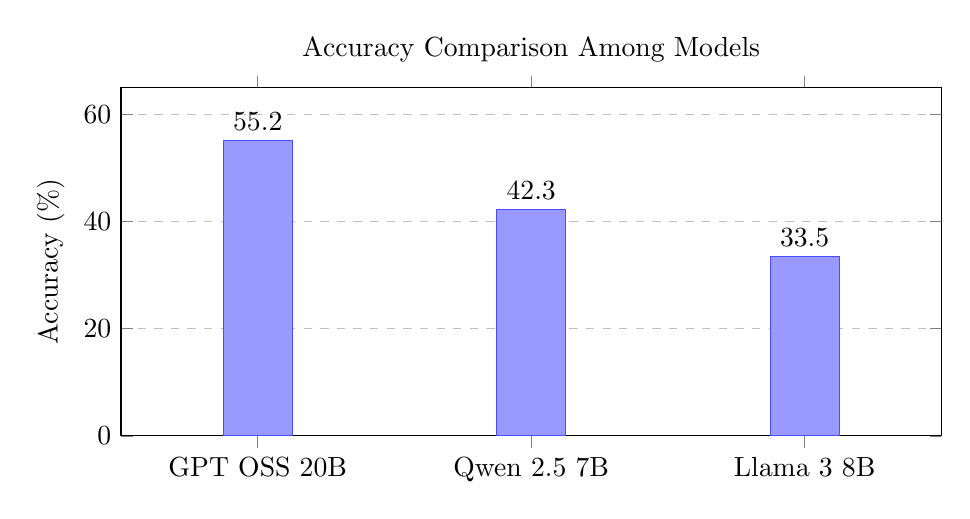
\begin{tikzpicture}
    \begin{axis}[
        ybar,
        width=12cm,              % Aumenta a largura total
        height=6cm,              % Diminui a altura total (achata o gráfico)
        enlarge x limits=0.25,
        legend style={at={(0.5,-0.25)}, anchor=north, legend columns=-1}, % Ajustado o -0.15 para -0.25 para não sobrepor o eixo X achatado
        ylabel={Accuracy (\%)},
        symbolic x coords={GPT OSS 20B, Qwen 2.5 7B, Llama 3 8B},
        xtick=data,
        nodes near coords,
        nodes near coords align={vertical},
        ymin=0, ymax=65, 
        bar width=25pt,          % Se o gráfico ficar muito apertado, diminua este valor (ex: 18pt)
        title={Accuracy Comparison Among Models},
        ymajorgrids=true,
        grid style=dashed,
    ]
        \addplot[fill=blue!40, draw=blue!70] coordinates {
            (GPT OSS 20B, 55.2) 
            (Qwen 2.5 7B, 42.3) 
            (Llama 3 8B, 33.5)
        };
    \end{axis}
\end{tikzpicture}
    }
    \caption{Accuracy results obtained.}
    % \caption{Resultados de acurácia obtidos pelo   {NoseSense} na detecção de  {test smells}.}
    \label{fig:grafico_modelos}
    \vspace{-10px}
\end{figure}

The tool's efficacy in providing diagnostics subsidies for LLMs is proven by analyzing the generated artifacts. Through the Detectability Ranking, the system accurately identified which anomalies are more "visible" to current semantic understanding; the Exception Catching Throwing category, for example, showed high detectability (87.3\%), contrasting with Ignored Test, which emerged as the greatest challenge for the models (14.7\%).
% A eficácia da ferramenta em fornecer subsídios para o diagnóstico de LLMs é comprovada pela análise dos artefatos gerados. Através do Ranking de Detectabilidade, o sistema identificou com precisão quais anomalias são mais "visíveis" para a compreensão semântica atual; a categoria  {Exception Catching Throwing}, por exemplo, apresentou alta detectabilidade (89,3\%), contrastando com  {Ignored Test}, que se consolidou como o maior desafio para os modelos (18,0\%). 

Regarding Performance Discrimination, NoseSense was able to rank the models by accuracy, pointing to GPT OSS 20B as the most effective on the proposed dataset (55.2\%) and Llama 3 8B as the least accurate (33.5\%). Finally, the platform consolidated comprehensive statistical reports, including a 43.7\% average accuracy and a 8.9\% standard deviation among the models, allowing for immediate scientific data interpretation after test completion.
% Quanto à Discriminação de Performance, o   {NoseSense} foi capaz de ranquear os modelos por acurácia, apontando o  {GPT OSS 20B} como o mais eficaz no  {dataset} proposto (55,2\%) e o  {Llama 3 8B} como o menos preciso (33,5\%). Por fim, a plataforma consolidou relatórios estatísticos abrangentes, incluindo uma acurácia média de 43,7\% e um desvio padrão de 8,9\% entre os modelos, permitindo uma interpretação científica imediata dos dados após a conclusão dos testes.

\subsection{Multiclass Confusion Analysis}
% \subsection{Análise de Confusão Multiclasse}
\label{subsec:confusion_analysis}

Beyond aggregate accuracy, a deeper understanding of model behavior requires analyzing how misclassifications are distributed across categories. To this end, NoseSense generates a multiclass confusion matrix that cross-references actual test smell labels with the classifications produced by the LLMs. Since the multiple-choice options are randomized per sample, the system resolves each model response back to the corresponding smell name before aggregation. Table~\ref{tab:confusion_matrix} presents the aggregated confusion matrix for the three evaluated models.
% Além da acurácia agregada, uma compreensão mais profunda do comportamento dos modelos requer a análise de como as classificações incorretas se distribuem entre as categorias. Para esse fim, o NoseSense gera uma matriz de confusão multiclasse que cruza os rótulos reais dos test smells com as classificações produzidas pelas LLMs. Como as opções de múltipla escolha são randomizadas por amostra, o sistema resolve cada resposta do modelo de volta ao nome do smell correspondente antes da agregação. A Tabela~\ref{tab:confusion_matrix} apresenta a matriz de confusão agregada para os três modelos avaliados.

% (Actual $\times$ Predicted) Diagonal values (in bold) represent correct classifications. The ``None'' column indicates samples where the model selected the ``None of the above'' option.
\begin{table}[htb]
    \centering
    \caption{Aggregated Multiclass Confusion Matrix}
    \label{tab:confusion_matrix}
    \renewcommand{\arraystretch}{1.150}
    \footnotesize
    \resizebox{\columnwidth}{!}{%
    \begin{tabular}{l|cccccccccc|c}
        \toprule
        \textbf{} & \textbf{AR} & \textbf{CTL} & \textbf{DA} & \textbf{ET} & \textbf{ECT} & \textbf{IT} & \textbf{MN} & \textbf{SE} & \textbf{UT} & \textbf{VT} & \textbf{None} \\
        \midrule
        AR         & \textbf{133} &   6 &  24 &  26 &  13 &   7 &  22 &   8 &   4 &   6 &  51 \\
        CTL     &  12 & \textbf{117} &  28 &  20 &  26 &   5 &  16 &   4 &   7 &  26 &  39 \\
        DA            &  14 &   8 & \textbf{199} &  17 &   9 &   3 &  10 &   2 &   3 &  13 &  22 \\
        ET                  &   4 &   2 &  10 & \textbf{89} &  26 &   1 &  17 &   5 &   8 &  14 & 124 \\
        ECT    &   1 &   3 &   3 &   4 & \textbf{262} &   1 &   1 &   0 &   3 &   0 &  22 \\
        IT                &  16 &   7 &  18 &  26 &  35 & \textbf{44} &  21 &   4 &  11 &  21 &  97 \\
        MN           &   9 &   2 &  17 &  24 &  23 &   4 & \textbf{122} &   6 &   5 &  16 &  72 \\
        SE          &  14 &   7 &  14 &   9 &  25 &   3 &  20 & \textbf{108} &   5 &   5 &  90 \\
        UT                &  10 &  10 &  14 &  26 &  24 &   8 &  19 &   6 & \textbf{69} &   5 & 109 \\
        VT                &  12 &   3 &  13 &  23 &  17 &   8 &  17 &   3 &   6 & \textbf{167} &  31 \\
        \bottomrule
    \end{tabular}
    }
\end{table}

The confusion matrix reveals several notable misclassification patterns. The ``None'' column is particularly informative: categories such as Eager Test (124), Unknown Test (109), Ignored Test (97), and Sensitive Equality (90) exhibit high rates of ``None'' selections, suggesting that the models frequently fail to recognize these anti-patterns entirely rather than confusing them with other smells. In contrast, Exception Catching Throwing shows minimal ``None'' selections (22), consistent with its high overall accuracy.
% A matriz de confusão revela vários padrões notáveis de classificação incorreta. A coluna ``None'' é particularmente informativa: categorias como Eager Test (124), Unknown Test (109), Ignored Test (97) e Sensitive Equality (90) exibem altas taxas de seleções ``None'', sugerindo que os modelos frequentemente falham em reconhecer esses antipadrões por completo, em vez de confundi-los com outros smells. Em contraste, Exception Catching Throwing mostra seleções ``None'' mínimas (22), consistente com sua alta acurácia geral.

To provide a more rigorous evaluation beyond simple accuracy, Table~\ref{tab:precision_recall} presents the per-class Precision, Recall, and F1-Score metrics derived from the confusion matrix. Precision measures the proportion of correct predictions among all samples classified as a given category, while Recall corresponds to the proportion of actual instances that were correctly identified.
% Para fornecer uma avaliação mais rigorosa além da simples acurácia, a Tabela~\ref{tab:precision_recall} apresenta as métricas de Precisão, Recall e F1-Score por classe derivadas da matriz de confusão. A Precisão mede a proporção de predições corretas entre todas as amostras classificadas como uma determinada categoria, enquanto o Recall corresponde à proporção de instâncias reais que foram corretamente identificadas.

\begin{table}[htb]
    \centering
    \caption{Per-class Accuracy, Precision, Recall, and F1-Score}
    \label{tab:precision_recall}
    \renewcommand{\arraystretch}{1.2}
    \footnotesize
    \begin{tabular}{lcccc}
        \toprule
        \textbf{Test Smell} & \textbf{Acc.} & \textbf{Prec.} & \textbf{Rec.} & \textbf{F1} \\
        \midrule
        ECT & 92.1\% & 57.0\% & 87.3\% & 68.9\% \\
        DA      & 91.9\% & 58.5\% & 66.3\% & 62.2\% \\
        VT          & 92.0\% & 61.2\% & 55.7\% & 58.3\% \\
        AR    & 91.4\% & 59.1\% & 44.3\% & 50.7\% \\
        CTL      & 92.3\% & 70.9\% & 39.0\% & 50.3\% \\
        SE    & 92.3\% & 74.0\% & 36.0\% & 48.4\% \\
        MN     & 89.3\% & 46.0\% & 40.7\% & 43.2\% \\
        ET            & 87.1\% & 33.7\% & 29.7\% & 31.6\% \\
        UT          & 90.6\% & 57.0\% & 23.0\% & 32.8\% \\
        IT          & 90.1\% & 52.4\% & 14.7\% & 22.9\% \\
        \midrule
        \textbf{Macro Avg.}   & \textbf{90.9\%} & \textbf{57.0\%} & \textbf{43.7\%} & \textbf{46.9\%} \\
        \bottomrule
    \end{tabular}
\end{table}


Per-category analysis reveals an asymmetry between Precision and Recall: the Sensitive Equality and Conditional Test Logic classes achieve high precision (reliable predictions) but low recall (many instances go undetected). The opposite occurs with Exception Catching Throwing, which presents high recall (few omissions) but moderate precision due to false positives. The macro F1-Score of 46.9\% confirms that while there is reasonable detection capability in some scenarios, there remains significant room for improvement, especially for Ignored Test and Eager Test. These results reinforce the role of NoseSense as a diagnostic instrument, as the confusion analysis maps the semantic boundaries where LLMs fail, offering actionable insights for prompt engineering refinement and model selection.

% The analysis of per-class metrics reveals an important asymmetry between Precision and Recall across categories. Sensitive Equality (74.0\%) and Conditional Test Logic (70.9\%) achieve the highest precision values, indicating that when the models classify a sample as belonging to these categories, the prediction is reliable. However, their corresponding recall values are substantially lower (36.0\% and 39.0\%, respectively), meaning that many actual instances go undetected. Conversely, Exception Catching Throwing achieves the highest recall (87.3\%) but moderate precision (57.0\%), suggesting that while the models rarely miss this pattern, they also incorrectly assign other smells to this category.
% The macro-averaged F1-Score of 46.9\% provides a balanced summary of model performance that accounts for both precision and recall, confirming that while the models demonstrate reasonable capability in certain categories, there remains significant room for improvement, particularly for Ignored Test (F1 = 22.9\%) and Eager Test (F1 = 31.6\%). These findings reinforce the value of NoseSense as a diagnostic instrument: beyond simple accuracy rankings, the confusion analysis reveals the specific semantic boundaries where current LLMs struggle, providing actionable insights for prompt engineering refinement and model selection.

% \subsection{Pipeline Stability and Reliability}
% \subsection{Estabilidade e Confiabilidade do Pipeline}

% The proof of concept validated three critical architectural aspects for the viability of large-scale experiments. First, the request resilience was ensured through semaphores and concurrency control, allowing the 3,000 calls to be completed without rate limiting failures. Second, the SSE flow integrity ensured real-time synchronization between frontend and backend, proving the streaming protocol's efficacy for long-duration experiment monitoring. And third, the full persistence of logs and responses in the \texttt{SQLite} database ensured the necessary traceability for auditing and test reproducibility in accordance with the rigor required in academic research. In short, the experiment confirms that NoseSense fulfills its purpose of being an agile and reliable infrastructure, transforming manual AI evaluation processes into an automated, measurable workflow prepared for state-of-the-art LLMs.
% A prova de conceito validou três aspectos arquiteturais críticos para a viabilidade de experimentos em larga escala. Primeiramente, a resiliência das requisições foi assegurada pelo uso de semáforos e controle de concorrência, permitindo que as 3.000 chamadas fossem concluídas sem falhas de rate limiting. Adicionalmente, a integridade do fluxo SSE garantiu a sincronia em tempo real entre frontend e backend. Por fim, a persistência integral de logs e respostas no banco de dados SQLite garantiu a rastreabilidade necessária para auditoria e a reprodutibilidade dos testes. Em suma, o experimento confirma que o NoseSense cumpre seu propósito de ser uma infraestrutura ágil e confiável.

\section{Related Works}

The rapid advancement of LLMs has driven the development of benchmarking tools, such as promptfoo, which, like NoseSense, enables the comparison of multiple models. They share a focus on local and integrated execution, offering an automated environment for validation and analytical report generation \cite{webster2023promptfoo,shankar2024validates,10.1145/3772318.3790897}.

% The rapid advancement of Large Language Models (LLMs) has driven the development of specialized tools for automated evaluation and continuous benchmarking, with promptfoo emerging as a prominent example \cite{webster2023promptfoo}. Both NoseSense and promptfoo converge by enabling the comparisons of multiple state-of-the-art models (e.g. OpenAI, Meta, and Anthropic), using data-driven analysis. They share a focus on local and integrated execution, offering developers a controlled environment capable of automating validations and generating consolidated analytical reports \cite{webster2023promptfoo,shankar2024validates,10.1145/3772318.3790897}.

The main divergence between the two tools lies in specialization: promptfoo has a broad, general-purpose focus, whereas NoseSense is highly specific to test smell detection. NoseSense is based on a validated 1,000-sample oracle labeled by JNose~\cite{virginio2020jnose}, a structured CRISPE-based prompt engine tailored to test smell taxonomy, and a custom analytical dashboard that produces domain-relevant metrics, per-category accuracy, multiclass confusion matrices, alongside per-class Precision, Recall, and F1-Score, which promptfoo does not natively provide \cite{webster2023promptfoo,shankar2024validates,10.1145/3772318.3790897}.



% Despite these operational similarities, the tools diverge significantly in focus and practical scope. The key distinction lies in specialization: while promptfoo is broad and general-purpose, NoseSense occupies a highly specific niche dedicated to test smell detection. Although it is theoretically possible to replicate NoseSense's functionality in promptfoo by providing a custom dataset and hand-crafting evaluation assertions, doing so requires substantial configuration effort and yields no domain-specific analytical support. NoseSense removes this burden by embedding, out of the box, a validated 1,000-sample oracle labeled by JNose~\cite{virginio2020jnose}, a structured CRISPE-based prompt engine tailored to test smell taxonomy, and a purpose-built analytical dashboard that produces domain-relevant metrics , per-category accuracy, multiclass confusion matrices, per-class Precision, Recall, and F1-Score , which promptfoo does not natively provide. 

Furthermore, NoseSense integrates real-time SSE-based monitoring specifically designed for long-running LLM inference sessions, whereas promptfoo targets shorter prompt evaluation cycles. In summary, NoseSense does not compete with promptfoo as a general benchmarking framework; rather, it delivers a ready-to-use, zero-configuration instrument that allows researchers to immediately evaluate any newly released model against an established software quality oracle, without requiring expertise in prompt engineering or dataset curation \cite{webster2023promptfoo,shankar2024validates,10.1145/3772318.3790897}.

\section{Threats to Validity}
\label{sec:ameacas}

We identified several threats to the validity of our study, organized according to established categories~\cite{wohlin2024experimentation}.


\textbf{Construct Validity:} Our prompt engineering strategy utilized a single template style, CRISPE, which may limit the generalizability of our conclusions. The multiple-choice format restricts the models' response space and may introduce bias, as models are guided to choose from predefined alternatives.

% \textbf{Construct Validity.} Our prompt engineering strategy utilized a single template style (CRISPE with multiple-choice options), which may limit the generalizability of our conclusions. The multiple-choice format restricts the models' response space and may introduce bias, as models are guided to choose from predefined alternatives rather than generating a classification freely. Furthermore, while randomizing the order of alternatives mitigates position bias, it does not eliminate it entirely.

\textbf{Internal Validity:} Our metrics are based on a single execution per sample for each model. Since LLMs are inherently non-deterministic, repeated executions of the same prompt may yield different responses. The absence of multiple runs limits our ability to measure response variance. Additionally, the use of default hyperparameters for model inference may influence the determinism of the generated responses.

% \textbf{Internal Validity.} The reported accuracy and F1 metrics are based on a single execution per sample per model. Since LLMs are inherently non-deterministic, repeated executions of the same prompt may yield different responses. The absence of multiple runs limits our ability to measure response variance and may affect the stability of the reported numbers. Additionally, the use of default hyperparameters for model inference (such as temperature and top-p) might further influence the quality and determinism of the generated responses. We acknowledge this as a limitation of the proof-of-concept evaluation; future studies using NoseSense should incorporate multiple runs to derive more robust estimates.



\textbf{External Validity:} Due to our choice of Java, our data may not generalize to other programming languages. The oracle dataset is subject to the constraints of the JNose tool. Furthermore, the evaluation dataset represents only a limited sample of the real world, and results may vary across other project domains.


% \textbf{External Validity:} There is a programming language limitation since we evaluated only Java code. Although Java is the most referenced language in the test smell literature, the results may not generalize to other programming languages. The oracle dataset, composed of 1,000 instances extracted and labeled using JNose~\cite{virginio2020jnose}, is subject to the accuracy constraints of that static analysis tool. JNose applies rule-based heuristics to identify test smells, meaning any false positives or false negatives in its detections propagate into our ground truth. While this approach ensures consistency with established definitions in the literature, it may not capture all nuanced instances of each smell type. Finally, the evaluation dataset represents a limited sample of the diversity of real-world test code patterns, and results may vary across different software domains or project types.

\textbf{Conclusion Validity:} No qualitative study was conducted to evaluate the tool with end-users to verify reduction of effort, results, usability metrics, or evaluations based on real-world tasks.

% \textbf{Conclusion Validity:} The tool was not evaluated with actual users. Although NoseSense is designed to improve the workflow of researchers conducting LLM benchmarking, no user study was carried out to assess whether it effectively reduces effort, time, or errors compared to manual or ad-hoc evaluation setups. The absence of usability metrics or task-based evaluations limits the extent to which we can claim productivity improvements for researchers. Future work should include controlled experiments or qualitative studies with researchers in the software engineering community to validate the practical utility of the tool.


\section{Conclusion}
% \section{Conclusão}
\label{sec:conclusao}


This paper presented NoseSense, a dynamic benchmarking tool designed to address the rapid obsolescence of traditional static studies evaluating LLMs. By shifting from time-consuming, static analyses to a pragmatic, real-time validation platform, NoseSense provides a continuous and reliable metrology instrument for assessing AI efficacy in test smell detection.
% Este artigo apresentou o NoseSense, uma ferramenta de benchmarking dinâmico projetada para solucionar a rápida obsolescência dos estudos estáticos tradicionais que avaliam Grandes Modelos de Linguagem (LLMs) na Engenharia de Software. Ao mudar o foco de análises pontuais e demoradas para uma plataforma pragmática de validação em tempo real, o NoseSense fornece um instrumento de metrologia contínuo e confiável para avaliar a eficácia da IA na detecção de test smells.

Through its layered architecture and the use of low-latency communication protocols like SSE, the tool efficiently orchestrates the simultaneous execution of heterogeneous LLMs. Our empirical demonstration, encompassing an automated evaluation pipeline and a comprehensive data visualization environment for 10 distinct test smell categories, proves NoseSense's utility in simplifying the interpretation of complex benchmarking results. NoseSense helps reduce the barrier for researchers and engineers to make empirically informed decisions about the selection of the model for software quality assurance.
% Por meio de sua arquitetura em camadas e do uso de protocolos de comunicação de baixa latência como Server-Sent Events (SSE), a ferramenta orquestra com eficiência a execução simultânea de LLMs heterogêneos. Além disso, nossa demonstração empírica comprova a utilidade do NoseSense em simplificar a interpretação de resultados complexos de benchmarking. Em última análise, o NoseSense reduz a barreira para que pesquisadores e engenheiros tomem decisões empiricamente fundamentadas sobre a seleção de modelos para garantia de qualidade de software.

\section*{Artifact Availability}

The NoseSense tool, including its source code, oracle dataset, and replication package, is publicly available at: \url{https://doi.org/10.5281/zenodo.22149462} and \url{https://github.com/arieslab/NoseSense} under the MIT License.
% A ferramenta NoseSense, incluindo seu código-fonte, dataset oráculo e pacote de replicação, está disponível publicamente em: \url{https://github.com/maccedoz/NoseSense}.

%% The next two lines define the bibliography style to be used, and
%% the bibliography file.
\bibliographystyle{ACM-Reference-Format}
\bibliography{bibartigotools}

%% If your work has appendices, this is the place to put them

\end{document}

% ============================================================
% CBSoft ACM-like Template – Author Checklist
% ============================================================
%
% 1. Remove CCS Concepts
%    - Remove the CCSXML block and \ccsdesc commands.
%
% 2. Remove ACM footer
%    Use the command \renewcommand\footnotetextcopyrightpermission[1]{}
%
% 3. Remove ACM Reference Format
%    Use the commands \setcopyright{none} and 
%    \settopmatter{printacmref=false}
%
% 4. Short title must not exceed column width
%    Use the command 
%    \renewcommand{\shorttitle}{The Name of the Title Is Hope}
%
% 5. Include authors' surnames in the page headers (even pages)
%    - The author names in the page header (at the top of the page)
%      must not exceed the column width
%    - This list must contain only the authors' surnames
%    - Suggestion: use "Surname et al." for more than two authors with the
%      command \renewcommand{\shortauthors}{Surname1stAuthor et al.}
%
% 6. Author format below title:
%    \author{FirstName Surname}
%    \affiliation{
%      \institution{Department, Institution}
%      \city{City}
%      \country{Country}}
%    \email{email@email.com}
%
% 7. Verify all author emails are included
%    - Check font consistency
%
% 8. All numbered section and subsection titles must follow the same
%    capitalization style: the first letter of each word in the title 
%    must be capitalized (Title Case).
%
% 9. Artifact Availability (check CFP)
%    - Not numbered -- use \section*{Artifact Availability}
%    - Placed after Conclusion and before Acknowledgments
%    - In Portuguese, use \section*{Disponibilidade de Artefatos}
